\documentclass[12pt]{article}
\setlength{\textwidth}{17cm}
\setlength{\textheight}{24cm}
\setlength{\topmargin}{-2cm}
\setlength{\footskip}{1cm}
\setlength{\evensidemargin}{0cm}
\setlength{\oddsidemargin}{0cm}
\setlength{\parindent}{0cm}

\usepackage{allrunes}
\usepackage{amsmath}
\usepackage[magyar]{babel}
\usepackage[T1]{fontenc}
\usepackage[utf8]{inputenc}
\usepackage{fixltx2e}
\usepackage{multirow}

\usepackage[hyphens]{url}
\usepackage[unicode,colorlinks=true,breaklinks]{hyperref}
%\usepackage[dvips]{hyperref}
%should display links, but it does not work with \H accent
%and formulas in section titles

\hypersetup{colorlinks,linkcolor=blue,urlcolor=magenta,citecolor=magenta}
%Breaks long url`s in text, while keeping it one link:

\usepackage{amsfonts}
\usepackage{amsthm}
\usepackage{amssymb}


\theoremstyle{plain}
\usepackage{graphicx}

%\usepackage{gensymb}
\usepackage{float}

% For bra-ket notation
\usepackage{braket}

%% New commands
\newcommand{\dd}{\textrm{d}}

%% Pauli matrices
\newcommand{\sigx}{\sigma_x}
\newcommand{\sigy}{\sigma_y}
\newcommand{\sigz}{\sigma_z}

\newcommand{\paulix}{
    \left( \begin{array}{cc}
        0 & 1 \\
        1 & 0
    \end{array}
    \right)
}

\newcommand{\pauliy}{
    \left( \begin{array}{cc}
        0 & -i \\
        i & 0
    \end{array}
    \right)
}

\newcommand{\pauliz}{
    \left( \begin{array}{cc}
        1 & 0 \\
        0 & -1
    \end{array}
    \right)
}


\begin{document}
\title{Valamelyik tétel}
\author{Nagy Dániel}


\maketitle
% \vspace*{7.5cm}
% \begin{figure}[h!]
%     \begin{center}
%     \includegraphics[width=0.4\textwidth]{./media/elte.eps}
%     \end{center}
% \end{figure}

\newpage

\section{Fejezet címe}
Random tétel

\subsection{Hasznos dolgok}
\begin{itemize}

    \item Minden képet, egyéb anyagot rakjunk a \texttt{<tétel száma>/media} mappába!
    \item Egy szimpla kép \ref{fig:tsneplot}.
    \begin{figure}[H]
        \begin{center}
        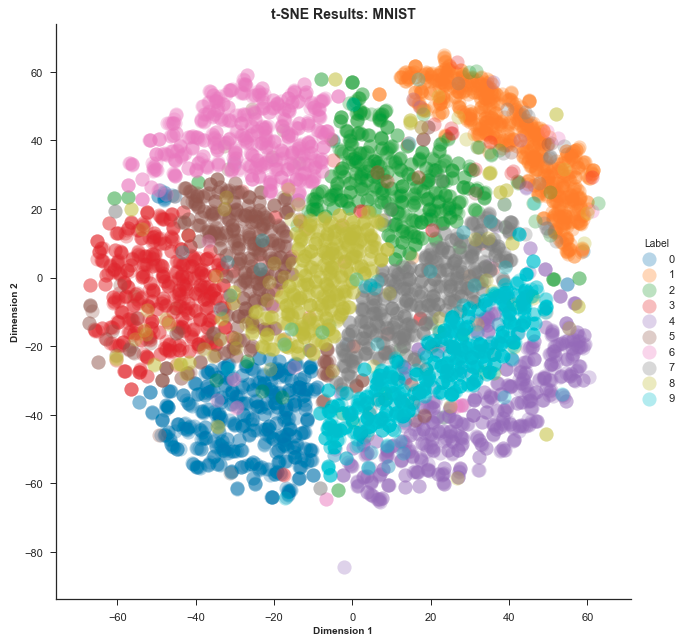
\includegraphics[width=0.5\textwidth]{media/tsneplot.png}
        \caption{t-SNE plot for MNIST dataset \cite{tsne-article}} 
        \label{fig:tsneplot}
        \end{center}
    \end{figure}

    \item Két kép egymás mellett:
    \begin{figure}[H]
        \centering
        \begin{minipage}{0.47\textwidth}
          \centering
          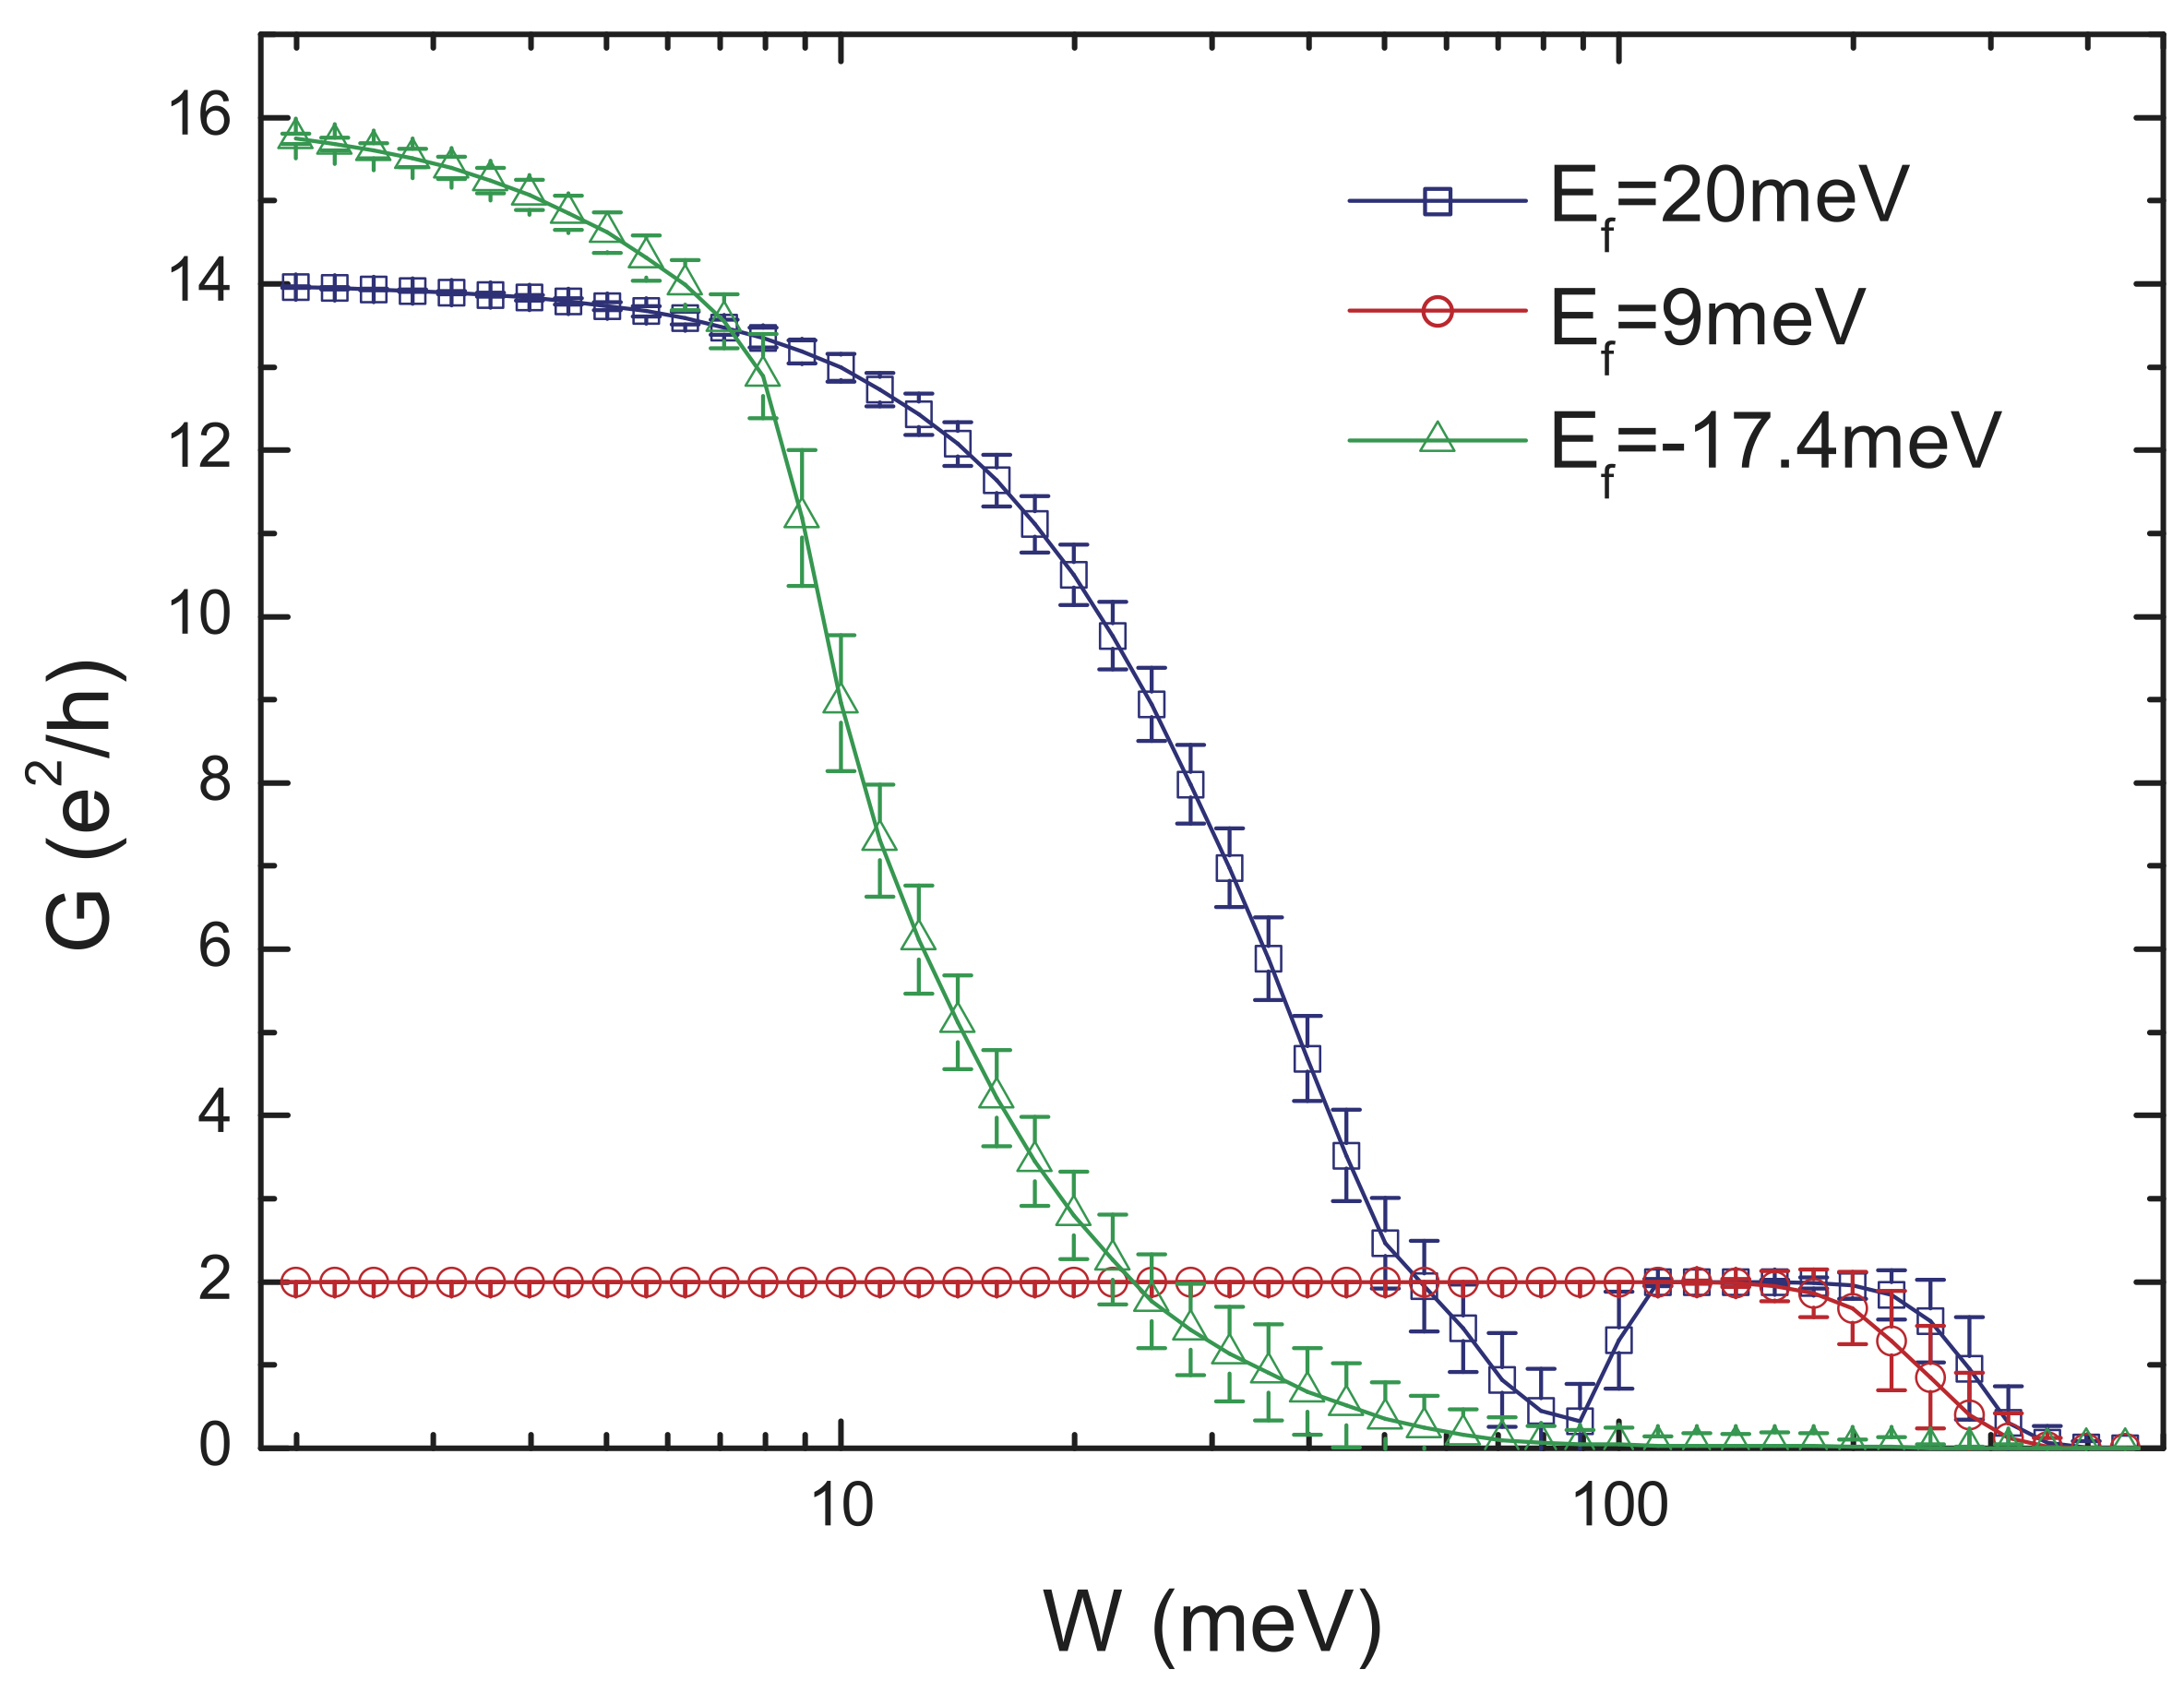
\includegraphics[width=1.0\textwidth]{./media/tai_results_from_article.png}
          \caption{Első kép}
      \end{minipage}\hfill
        \begin{minipage}{0.53\textwidth}
            \centering
            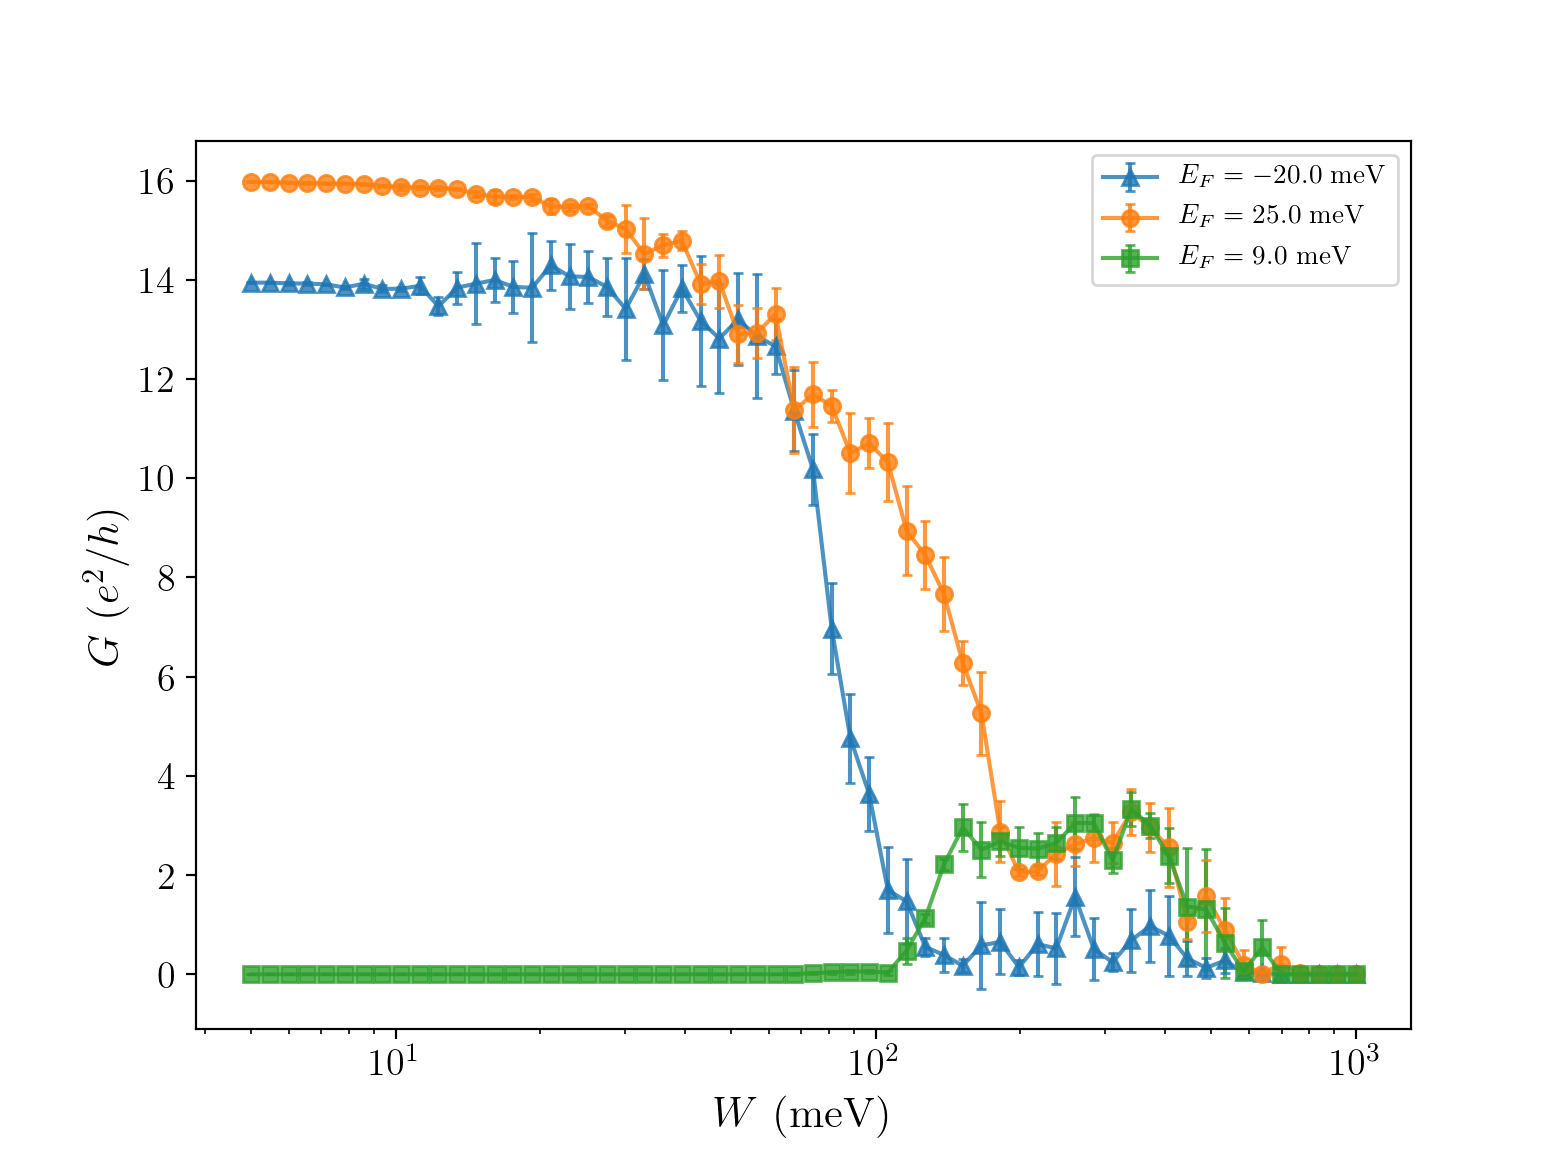
\includegraphics[width=1.0\textwidth]{./media/tai_results_params1_nsamples=4.png}
            \caption{Második kép}
        \end{minipage}
      \end{figure}

    \item Ez lesz egy url (hosszú url is jól működik): \url{https://towardsdatascience.com/time-series-analysis-and-climate-change-7bb4371021e}.
    
    \item Egy egyszerű képlet számozva:
    \begin{equation}
        (i\hbar\gamma^{\mu}\partial_{\mu} - mc)\ket\psi = 0
        \label{eq:dirac}
    \end{equation}
    Így hivatkozom: Dirac-egyenlet (\ref{eq:dirac}).

    \item Egy számozatlan képlet:
    \begin{equation*}
        \hat F (\omega) = \frac{1}{\sqrt{2\pi}} \int\limits^{\infty}_{-\infty} \dd t e^{-i\omega t}f(t) 
    \end{equation*}

    \item bra-ket jelölés: $\ket a \bra b \braket{a|b|c} \Braket{\psi|\sum\limits_{j=1}^{\infty} c_j | \psi}$
    
    \item Deriválásnál, integrálnál használjuk az egyenes $\dd$ (\texttt{\textbackslash dd}) parancsot: 
    \begin{equation*}
        \int \dd \omega \frac{\dd y}{\dd x}
    \end{equation*}

    \item Több összefüggés egymás alatt: \texttt{\textbackslash begin\{align*\} ... \textbackslash end\{align*\}}
    \begin{align*}
        &[b_l, b^\dagger_m] = \delta_{lm} \\
        &[b^\dagger_l, b^\dagger_m] = [b_l,b_m]=0 \textrm{,}
    \end{align*}

    \item Hosszú, többsoros képlet:
    \begin{align*}
        & A = B + C + D   \\
        & = \int \dd x f_B(x) + \int \dd x f_C(x) + \int \dd x f_D(x) \\
        & = 1-\frac{1}{\sqrt{2\pi}}\int \dd\omega Y(\omega)
    \end{align*}  
    
    \item Ha kódot szeretnénk képpé alakítani, itt egy hasznos tool \url{https://carbon.now.sh/?bg=rgba(171%2C184%2C195%2C0)&t=monokai&wt=none&l=python&ds=false&dsyoff=20px&dsblur=68px&wc=true&wa=true&pv=8px&ph=5px&ln=false&fm=Source%20Code%20Pro&fs=14px&lh=133%25&si=false&es=2x&wm=false}
    Eredmény:
    \begin{figure}[H]
        \begin{center}
        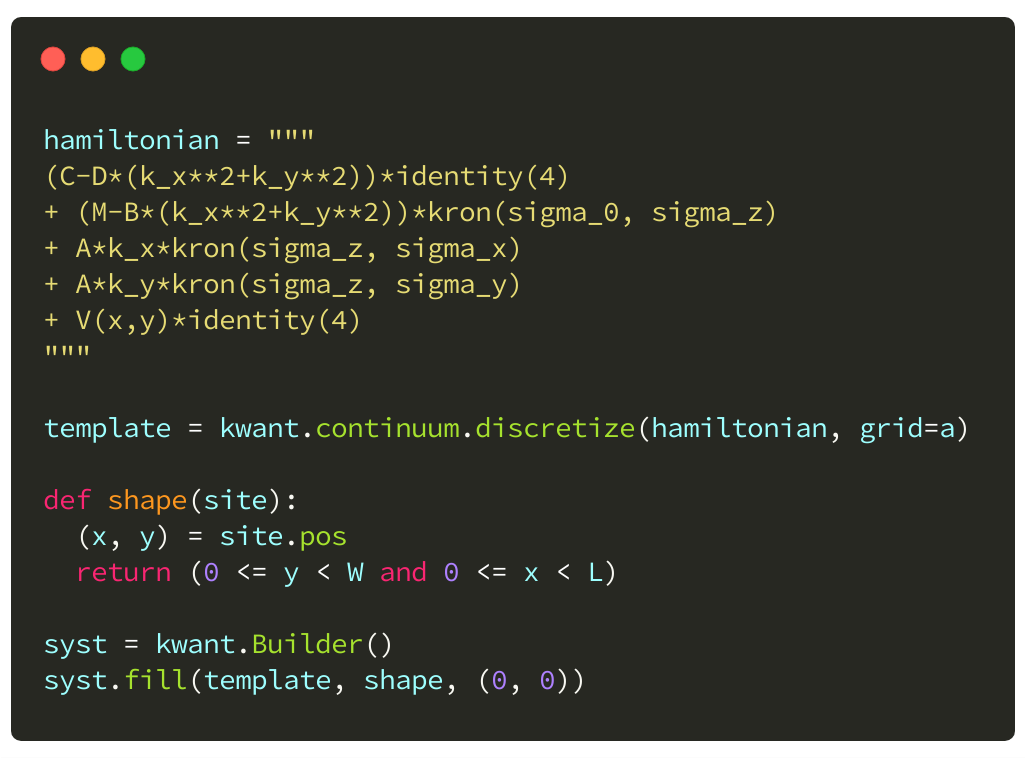
\includegraphics[width=0.6\textwidth]{media/hamilton_def.png}
        \caption{Kép forrása: \url{https://carbon.now.sh/}} 
        \end{center}
    \end{figure}
    \item Itt egy fizwebes referencia \cite{fizweb}.
    \item Itt meg a KNN wikipédia referencia \cite{knnwiki}.
\end{itemize}

\subsection{Blabla}

\bibliographystyle{plain}
\bibliography{references}

\end{document}
